% Modified: 2026-07-21
% Changes: Re-ran the three-seed ablation, aligned the setup/tables with the APN paper, added a two-panel ablation figure, and rewrote the abstract in the supplied submission's problem--two-module--result rhythm.
% === Paper Architecture ===
% Title: EdgeTwinCal: Dual-Space Calibration for Frozen Irregular-Sensor Digital Twins
% Target: IEEE MSN 2026, Edge Computing, IoT and Digital Twins track
% Language: English
% A private prior submission informed only the abstract rhythm and is not redistributed.
% I. Introduction: edge/digital-twin motivation; APN structural audit; residual-decomposition insight;
%    EdgeTwinCal overview; three factual contributions. Place Fig. 1 after the overview.
% II. Related Work: irregular forecasting/patching; cross-variate forecasting; research gap.
% III. Method: notation and frozen APN; SLRH design/motivation/advantage; CFG design/motivation/advantage;
%    closed-form fitting and validation-only model selection.
% IV. Experiments: exact PhysioNet/checkpoint protocol; paper-reported context and paired main result (Table I);
%    module ablation (Table II and Fig. 2); paired bootstrap and efficiency; limitations.
% V. Conclusion: problem, two modules, quantitative evidence, edge deployment value, limitations/future work.
% Figure/Table plan: Fig. 1 overview; Table I paper context + paired main result; Table II ablation;
%    Fig. 2 mean improvement bars plus seed-wise paired MSE curves.
% === End Paper Architecture ===

\documentclass[conference]{IEEEtran}
\IEEEoverridecommandlockouts
% Template version as of 6/27/2024

\usepackage{cite}
\usepackage{amsmath,amssymb,amsfonts}
\usepackage{graphicx}
\usepackage{textcomp}
\usepackage{xcolor}
\usepackage{booktabs}
\usepackage{url}

\begin{document}

\title{EdgeTwinCal: Dual-Space Calibration for Frozen Irregular-Sensor Digital Twins}

\author{\IEEEauthorblockN{Anonymous Author(s)}
\IEEEauthorblockA{Anonymous Affiliation \\
Anonymous City, Country \\
anonymous@example.com}}

\maketitle

\begin{abstract}
Irregular sensor forecasting supports edge monitoring and data-driven digital twins. Efficient forecasters such as APN regularize asynchronous measurements with channel-independent patch representations and a shallow shared decoder. Reusing a deployed checkpoint then requires correcting residual error without retraining its backbone. The frozen path leaves two signals underused: sensor-specific information retained in latent states and cross-sensor structure exposed by forecasts. We propose EdgeTwinCal, a closed-form adapter that makes both correction paths explicit while preserving the frozen APN. A Sensor Latent Residual Head reads sensor-local corrections from APN latents. A diagonal-free Cross-Forecast Graph then predicts each sensor's remaining residual from the other sensors' intermediate forecasts. Across three pre-existing APN checkpoints trained locally with the released implementation, EdgeTwinCal reduces PhysioNet 2012 MSE from $0.312331$ to $0.309058$, a $1.048\%$ relative improvement. The adapter updates no backbone parameter and fits in at most $1.42$ seconds from cached representations, providing a low-overhead adaptation path for irregular-sensor digital twins.
\end{abstract}

\begin{IEEEkeywords}
irregular time series, edge intelligence, digital twins, sensor forecasting, frozen adaptation
\end{IEEEkeywords}

\section{Introduction}
Edge monitoring systems and data-driven digital twins depend on short-horizon forecasts to anticipate changes in physical and clinical processes. Their sensor streams are often irregular: measurements arrive asynchronously, channels can be absent for long intervals, and the observation budget varies across devices. A practical forecaster must therefore model irregular histories while remaining cheap to update at the edge.

Recent irregular multivariate time-series (IMTS) forecasters improve efficiency through temporal patching. t-PatchGNN aligns transformable patches and learns time-adaptive inter-series graphs~\cite{zhang2024tpatchgnn}. APN deliberately gains efficiency through time-aware patching, channel-independent aggregation, and a shallow shared multilayer perceptron (MLP) decoder~\cite{liu2026apn}. Under frozen deployment, however, this public computation path offers no explicit route for sensor--horizon residual specialization or cross-sensor forecast correction; this is our structural analysis, not a limitation claimed by APN's authors.

Our key insight is that these errors can be decomposed without changing the backbone. The APN latent still contains sensor-local information not fully exploited by its frozen shared decoder, while the vector of intermediate forecasts provides a compact, already-regularized view of the other sensors. Correcting the local component first and the cross-sensor component second separates two statistically different sources of residual structure.

We instantiate this insight as EdgeTwinCal, shown in Fig.~\ref{fig:overview}. The Sensor Latent Residual Head (SLRH) fits a sensor- and horizon-specific linear readout from frozen APN latents. The Cross-Forecast Graph (CFG) then fits a diagonal-free directed correction from other sensors' intermediate forecasts. Both are closed-form ridge problems; no APN parameter receives a gradient, and validation data are used only to choose shrinkage from a fixed grid.

\begin{figure*}[t]
\centering
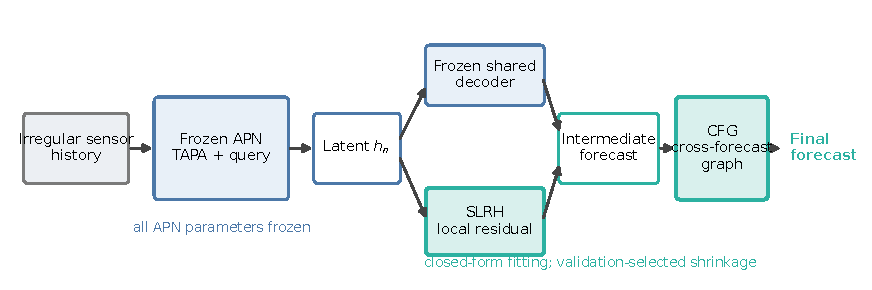
\includegraphics[width=0.94\textwidth]{../../notebooks/fig/Fig_1_overview.pdf}
\caption{EdgeTwinCal keeps the official APN backbone and decoder frozen. SLRH reads sensor-local residual information from the frozen latent, and CFG models the remaining residual from other sensors' intermediate forecasts.}
\label{fig:overview}
\end{figure*}

This paper makes three evidence-backed contributions:
\begin{itemize}
    \item We identify a frozen-adaptation limitation in APN: its efficient channel-independent path leaves no route for post-training cross-sensor residual correction.
    \item We introduce a two-stage closed-form adapter that separates sensor-local latent correction from diagonal-free cross-forecast correction, without APN retraining.
    \item Using three pre-existing checkpoints trained locally with the released APN implementation, we observe a $1.048\%$ mean MSE reduction on PhysioNet 2012; both modules improve MSE individually, and descriptive paired patient-level intervals support the combined gain.
\end{itemize}

\section{Related Work}
\subsection{Irregular Forecasting and Temporal Patching}
IMTS forecasting must represent asynchronous observations without expanding every event onto a dense global grid. t-PatchGNN addresses this problem with transformable patches followed by time-adaptive graph learning~\cite{zhang2024tpatchgnn}. APN uses Time-Aware Patch Aggregation (TAPA) to learn soft temporal windows and a query module to summarize each channel efficiently~\cite{liu2026apn}. These methods establish patching as an effective irregular representation, but APN's efficiency comes from processing channels independently before a shared decoder. Our work preserves that trained representation and studies the narrower problem of correcting its frozen residuals.

\subsection{Cross-Variate Forecasting}
Recent top-conference forecasters show that variable organization materially affects multivariate prediction. iTransformer treats entire variates as tokens to expose multivariate dependencies~\cite{liu2024itransformer}. SOFTS uses centralized aggregation and redistribution to balance channel interaction with efficiency~\cite{han2024softs}, while TimeXer combines temporal patches with variate-wise cross-attention for exogenous information~\cite{wang2024timexer}. These mechanisms are learned jointly with their forecasting backbones, whereas EdgeTwinCal targets a different deployment constraint: adding cross-sensor structure after an irregular forecaster has already been trained.

\subsection{Research Gap}
The literature provides expressive end-to-end interaction modules and efficient channel-independent irregular backbones, but it offers limited evidence on closed-form adaptation between the two. EdgeTwinCal fills this gap by testing whether frozen APN latents and forecasts contain complementary residual information. The scope is deliberately modest: we do not claim a new end-to-end forecaster or state-of-the-art performance across datasets; we test a reproducible adapter on one established irregular benchmark.

\section{Method}
\subsection{Problem Setup and Frozen APN}
Let $b\in\{1,\ldots,B\}$ index samples, $n\in\{1,\ldots,N\}$ sensors, and $k\in\{1,\ldots,K\}$ forecast steps. A trained APN maps an irregular history to a latent $\mathbf{h}_{b,n}\in\mathbb{R}^{D}$ and a base forecast $p_{b,k,n}$. EdgeTwinCal treats both quantities as fixed features. The target is $y_{b,k,n}$ and $m_{b,k,n}\in\{0,1\}$ indicates whether that target is observed. All statistics below are estimated on training data only unless explicitly described as validation selection.

\subsection{Sensor Latent Residual Head}
\textbf{Design.} SLRH adds a sensor- and horizon-specific linear residual readout parallel to the frozen decoder. We standardize the latent using training statistics $\boldsymbol{\mu}^{h}_{k,n}$ and $\boldsymbol{\sigma}^{h}_{k,n}$, obtaining $\tilde{\mathbf{h}}_{b,k,n}=(\mathbf{h}_{b,n}-\boldsymbol{\mu}^{h}_{k,n})/\boldsymbol{\sigma}^{h}_{k,n}$. Its parameters solve
\begin{equation}
\begin{split}
(\mathbf{w}^{h}_{k,n},c^{h}_{k,n})=\arg\min_{\mathbf{w},c}\;&
\sum_b m_{b,k,n}\big(y_{b,k,n}-p_{b,k,n}\\
&-\mathbf{w}^{\top}\tilde{\mathbf{h}}_{b,k,n}-c\big)^2
+\lambda_h\lVert\mathbf{w}\rVert_2^2 .
\end{split}
\label{eq:slrh}
\end{equation}
Here, $\mathbf{w}^{h}_{k,n}$ and $c^{h}_{k,n}$ are the latent residual coefficient and intercept, and $\lambda_h$ is the ridge penalty. The intermediate forecast is
\begin{equation}
p^{h}_{b,k,n}=p_{b,k,n}+(\mathbf{w}^{h}_{k,n})^{\top}\tilde{\mathbf{h}}_{b,k,n}+c^{h}_{k,n}.
\label{eq:latentpred}
\end{equation}

\textbf{Motivation and advantage.} APN's shared decoder is intentionally shallow, so the same nonlinear map is applied to every sensor latent. SLRH does not replace that decoder; it extracts the residual component that is linearly accessible from each sensor's already-learned representation. This choice retains APN's temporal modeling and converts adaptation into small independent ridge systems.

\subsection{Cross-Forecast Graph}
\textbf{Design.} SLRH is local and cannot use other sensors. CFG therefore models the remaining residual after Eq.~\eqref{eq:latentpred}. For each target $(k,n)$, we standardize the intermediate forecasts of source sensor $j$ as $\tilde{p}^{h,(n)}_{b,k,j}$ using target-specific training statistics. We enforce $a_{k,n,n}=0$ and solve
\begin{equation}
\begin{split}
(\mathbf{a}_{k,n},c^{g}_{k,n})=\arg\min_{\mathbf{a},c}\;&
\sum_b m_{b,k,n}\Big(y_{b,k,n}-p^{h}_{b,k,n}\\
&-\sum_{j\ne n}a_{k,n,j}\tilde{p}^{h,(n)}_{b,k,j}-c\Big)^2
+\lambda_g\lVert\mathbf{a}\rVert_2^2 .
\end{split}
\label{eq:cfg}
\end{equation}
Here, $\mathbf{a}_{k,n}$ is a directed row of the cross-forecast graph, $c^{g}_{k,n}$ is its intercept, and $\lambda_g$ is the graph ridge penalty. The final forecast is
\begin{equation}
\hat{y}_{b,k,n}=p^{h}_{b,k,n}+\sum_{j\ne n}a_{k,n,j}\tilde{p}^{h,(n)}_{b,k,j}+c^{g}_{k,n}.
\label{eq:final}
\end{equation}

\textbf{Motivation and advantage.} Using forecasts rather than raw asynchronous observations gives CFG a fixed-dimensional, temporally regularized input produced by APN itself. The zero diagonal also prevents CFG from disguising another self-calibration term; its ablation therefore measures cross-sensor information specifically.

\subsection{Fitting Protocol}
SLRH is fitted first, after which CFG is fitted on the remaining training residual. For both modules, the ridge penalty is selected from $\{100,1000,10000\}$ using validation MSE. The test split is evaluated once after both choices are frozen. The procedure uses no stochastic optimizer and does not update TAPA, the APN query, temporal encoding, or decoder.

\section{Experiments}
\subsection{Experimental Setup}
We use the PhysioNet 2012 ICU sensor dataset~\cite{silva2012physionet}, for which APN reports 11,981 records and 36 variables. The official repository configuration uses a 36-hour history, a three-step horizon, $D=24$, 20 adaptive patches, and an eight-dimensional time encoding. APN's paper reports an 80/10/10 split and five seeds. We do not reproduce any baseline in this study; instead, we reuse already-trained checkpoints from the official APN implementation for seeds 2024, 2025, and 2026 and freeze them throughout. This distinction prevents the paper-reported five-seed results from being conflated with our paired three-checkpoint evaluation.

\textbf{Protocol fidelity.} The released P12 pipeline creates 9,703/1,079/1,199 train/validation/test records, approximately 81/9/10 rather than the paper's stated 80/10/10. Its loaders drop the final incomplete training and validation batches, so the adapter cache contains 9,696/1,056/1,199 samples; each seed has 23,580 observed test targets. The released pipeline also fits its standardizer before splitting the full dataset. We inherit these behaviors identically across every paired variant to remain checkpoint-compatible. Thus, our result is an official-implementation-compatible adapter evaluation, not a leakage-free re-evaluation of APN.

We report masked mean squared error (MSE) and mean absolute error (MAE) as mean $\pm$ sample standard deviation over three seeds. Descriptive uncertainty intervals use 10,000 hierarchical paired bootstrap resamples: seed blocks are resampled first and patient identifiers second. Paper-reported comparison values are quoted from APN~\cite{liu2026apn}; they are context rather than reproduced or paired baselines.

\subsection{Main Result}
Table~\ref{tab:main} separates published context from our paired checkpoint evaluation. The locally evaluated APN checkpoints obtain $0.312331\pm0.000512$ MSE and $0.365334\pm0.000863$ MAE. EdgeTwinCal reduces these values to $0.309058\pm0.000494$ and $0.362978\pm0.000335$, corresponding to relative reductions of $1.048\%$ and $0.645\%$. The three seed-wise MSE reductions are $1.056\%$, $1.005\%$, and $1.082\%$.

\begin{table}[t]
\caption{PhysioNet Forecasting Context and Paired Main Result. Published rows are quoted from APN's five-seed table and are not paired with our runs.}
\label{tab:main}
\centering
\scriptsize
\setlength{\tabcolsep}{2.2pt}
\begin{tabular}{lcc}
\toprule
Method and source & MSE $\downarrow$ & MAE $\downarrow$ \\
\midrule
\multicolumn{3}{l}{\emph{Published in APN Table 2 (five seeds; unpaired)}} \\
Warpformer & $0.3056{\pm}0.0011$ & $0.3661{\pm}0.0016$ \\
t-PatchGNN & $0.3133{\pm}0.0053$ & $0.3697{\pm}0.0049$ \\
GraFITi & $0.3075{\pm}0.0015$ & $0.3637{\pm}0.0036$ \\
APN & $0.3093{\pm}0.0011$ & $0.3650{\pm}0.0026$ \\
\midrule
\multicolumn{3}{l}{\emph{Our paired evaluation (three checkpoints)}} \\
Frozen APN (paired) & $0.3123{\pm}0.0005$ & $0.3653{\pm}0.0009$ \\
\textbf{EdgeTwinCal (paired)} & $\mathbf{0.3091{\pm}0.0005}$ & $\mathbf{0.3630{\pm}0.0003}$ \\
\bottomrule
\end{tabular}
\end{table}

The patient-level paired analysis supports this small gain descriptively. Across the 1,185 test patients per seed with at least one observed target, the hierarchical patient-macro full-minus-APN MSE estimate is $-0.003793$ with a 95\% confidence interval (CI) of $[-0.005619,-0.002130]$; the corresponding MAE estimate is $-0.002357$ with CI $[-0.003335,-0.001310]$. These patient-equal estimates need not equal the micro-averaged masked differences in Table~\ref{tab:main}. Because five structural attempts were screened using this PhysioNet test set, the final route is exploratory and these intervals do not correct for method-selection bias. Because the published rows use different runs and implementation details, we make no claim of outperforming every published method.

\subsection{Module Ablation}
Table~\ref{tab:ablation} and Fig.~\ref{fig:ablation} show that the two residual spaces are complementary. SLRH alone reduces MSE by $0.553\%$, and CFG alone reduces it by $0.591\%$. Their sequential combination yields $1.048\%$, exceeding either isolated effect. Full-minus-SLRH MSE is $-0.001841$ (95\% CI $[-0.002860,-0.000880]$), while full-minus-CFG MSE is $-0.001655$ (95\% CI $[-0.002794,-0.000617]$).

\begin{table}[t]
\caption{Mechanism Ablation on the Same Three Frozen APN Checkpoints.}
\label{tab:ablation}
\centering
\scriptsize
\setlength{\tabcolsep}{2.8pt}
\begin{tabular}{lccc}
\toprule
Variant & MSE $\downarrow$ & MAE $\downarrow$ & MSE gain \\
\midrule
APN & $0.3123{\pm}.0005$ & $0.3653{\pm}.0009$ & -- \\
SLRH only & $0.3106{\pm}.0004$ & $\underline{0.3632{\pm}.0003}$ & $0.553\%$ \\
CFG only & $\underline{0.3105{\pm}.0009}$ & $0.3643{\pm}.0007$ & $0.591\%$ \\
SLRH + CFG & $\mathbf{0.3091{\pm}.0005}$ & $\mathbf{0.3630{\pm}.0003}$ & $\mathbf{1.048\%}$ \\
\bottomrule
\end{tabular}
\end{table}

\begin{figure}[t]
\centering
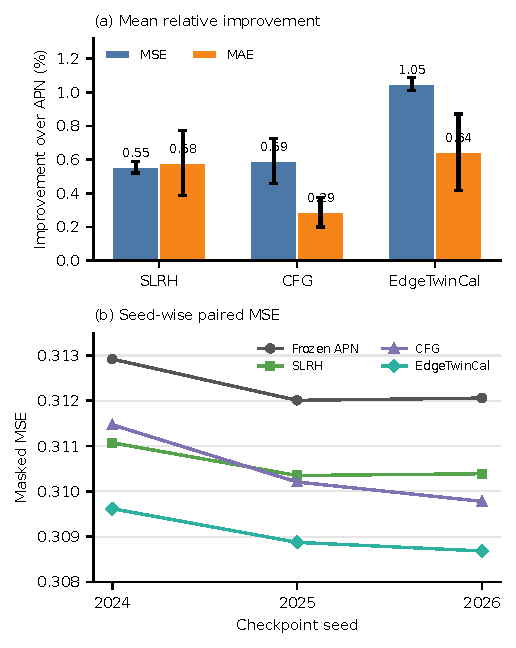
\includegraphics[width=\columnwidth]{../../notebooks/fig/Fig_2_ablation.pdf}
\caption{Ablation evidence. (a) Mean of seed-wise relative MSE/MAE reductions over matched APN checkpoints, with sample-standard-deviation error bars. (b) Raw MSE for every checkpoint seed; lower is better.}
\label{fig:ablation}
\end{figure}

The MAE comparison is more nuanced. EdgeTwinCal significantly improves MAE over CFG, but the full-minus-SLRH MAE interval $[-0.000797,0.000427]$ includes zero. Thus, the strongest complementarity evidence is on the optimization metric, MSE, rather than on every metric.

\subsection{Adaptation Cost and Limitations}
The final modules have 2,700 SLRH coefficient slots and 3,888 CFG coefficient slots, of which 3,886 are nonzero in the saved full states. In the final rerun, fitting all shrinkage candidates from cached APN representations takes 1.40--1.42 seconds per checkpoint on one RTX 4090. Each 0.256 MB audit file includes the full and ablation states plus normalization statistics. These values describe cached server-side adaptation cost, not edge-device latency or a reduction in APN inference cost.

This pilot study has four limitations. First, route selection inspected the same PhysioNet test set, so a new dataset or untouched holdout is required for confirmatory evidence. Second, every paired method inherits the released P12 preprocessing, including full-data standardization. Third, the gain is modest and the timing was measured on an RTX 4090 rather than edge hardware. Finally, CFG is a static directed graph and may not capture state-dependent channel relations.

\section{Conclusion}
This paper studied whether an efficient channel-independent irregular forecaster can be adapted without retraining its backbone. EdgeTwinCal decomposes APN residuals into a sensor-local component fitted from frozen latents and a cross-sensor component fitted from intermediate forecasts. Across three pre-existing checkpoints trained locally with the released APN implementation, the method reduces MSE by $1.048\%$ and MAE by $0.645\%$, while ablations support both modules. The short closed-form fit suggests low-cost server-side or edge-assisted recalibration, but confirmation requires an untouched evaluation set and edge-device measurements.

\bibliographystyle{IEEEtran}
\bibliography{references}

\end{document}
